\chapter{Laplace方程的格林函数法}
\thispagestyle{empty}
\section{Laplace方程边值问题的提出}
\subsection{三维Laplace方程}
\begin{equation}
	\nabla^2 u \equiv \dfrac{\partial^2 u}{\partial x^2} + \dfrac{\partial^2 u}{\partial y^2} + \dfrac{\partial^2 u}{\partial z^2} = 0
\end{equation}
三维Laplace方程的特点:
\begin{itemize}
	\item 描述稳定问题,即不随时间变化的过程,如热传导、扩
散、静电场等
	\item 只存在边界条件,无初始条件
	\item 一般有两种边值条件,构成两类边值问题
\end{itemize}
\vspace*{0.5em}

\subsection{两类边值问题}
\vspace*{-2em}
\begin{figure}[!htb]
	\centering
	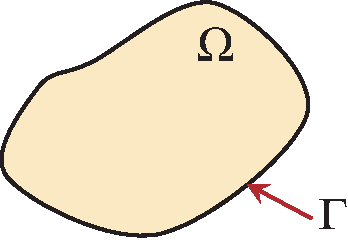
\includegraphics[width=0.2\linewidth]{pic/格林无点.pdf}
	\vspace*{-0.5em}
	\caption{空间区域}
	\label{格林1}
\end{figure}

\noindent \textbf{1. 第一边值问题(Dirichlet问题)}

如图\ref{格林1},在空间$(x,y,z)$中某一区域$\Omega$的边界$\Gamma$上给定连续函数$f$。

求一个函数$u(x,y,z)$,它在闭区域$\Omega+\Gamma$上等于已知函数$f$,即
\begin{equation}
	u\big|_{\Gamma} = f
\end{equation}
具有二阶连续偏导数并且满足Laplace方程的连续函数称为\dy[调和函数]{THHS}。所以,Dirichlet问题也可以描述为:

求一个函数$u(x,y,z)$,在$\Omega+\Gamma$上连续,在$\Omega$中是调和函数,它在边界$\Gamma$上的值为给定连续函数
\vspace*{1em}

\noindent \textbf{2. 第二边值问题(Neumann问题)}

如图\ref{格林1},在空间$(x,y,z)$中某一区域$\Omega$的边界$\Gamma$上给定连续函数$f$。

求一个函数$u(x,y,z)$,在$\Omega+\Gamma$上连续,在$\Omega$中是调和函数,它在边界$\Gamma$上任一点处法向导数存在且等于已知函数$f$,即
\begin{equation}
	\dfrac{\partial u}{\partial n}\Bigg|_{\Gamma} = f
\end{equation}
其中,$\bm{n}$是$\Gamma$的外法向量。
\vspace*{0.5em}

\subsection{内问题和外问题}

\noindent \textbf{1. 内问题}

在边界$\Gamma$上给定边界条件,在区域内部求Laplace方程的解,这样的问题称为\dy[内问题]{NWT}。
\vspace*{1em}

\noindent \textbf{2. 外问题}

在边界$\Gamma$上给定边界条件,在区域外部求Laplace方程的解,这样的问题称为\dy[外问题]{WWT}。

由于外问题是在无穷区域上给出的,在求解中常常要求附加条件:$\lim\limits_{r \to \infty} u(x,y,z) = u_0\quad (r = \sqrt{x^2 + y^2 + z^2})$

\section{格林公式}
\subsection{第一格林公式}
格林公式是曲面积分中高斯公式的直接推论。

\theorem[高斯公式]
如图\ref{格林2},设$\Omega$是一个足够光滑的、以曲面$\Gamma$为边界的有界区域,$\vec{U}$是在$\Omega + \Gamma$上连续的、在$\Omega$内有一阶连续的任意矢量函数,则有\dy[高斯公式]{GSGS}
\begin{equation}
	\iiint\limits_{\Omega} \nabla \cdot \vec{U} \, \d V = \iint \limits_{\Gamma} \vec{U} \cdot \, \d \vec{S}
\end{equation}
其中,$\d V$为体积元素,$\d \vec{S}$是$\Gamma$上的矢量面积微元,且$\d \vec{S}$的面元外法向为$\bm{n}$。

\begin{figure}[!htb]
	\centering
	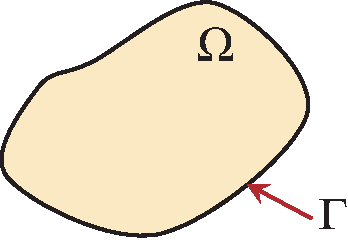
\includegraphics[width=0.2\linewidth]{pic/格林无点.pdf}
	\vspace*{-0.5em}
	\caption{空间区域}
	\label{格林2}
\end{figure}

\theorem[第一格林公式]
如图\ref{格林2},设函数$u(x,y,z)$和$v(x,y,z)$在$\Omega + \Gamma$上具有一阶连续偏导数,在$\Omega$内具有连续的所有二阶偏导数,取$\vec{U} = u \nabla v$,代入高斯公式可得\dy[第一格林公式]{DYGLGS}
\begin{equation}
	\iiint\limits_{\Omega}\big(u \nabla^2 v\big)\, \d V = \iint\limits_{\Gamma} u \dfrac{\partial v}{\partial n}\, \d S - \iiint\limits_{\Omega} \big(\nabla u \cdot \nabla v\big)\, \d V
	\label{GL1}
\end{equation}
其中,$\d V$为体积元素,$\d S$是$\Gamma$上的标量面积微元。
\vspace*{0.5em}

\subsection{第二格林公式}
\vspace*{-0.5em}
由第一格林公式\eqref{GL1},并交换$u$和$v$的位置,则有
\begin{equation}
	\iiint\limits_{\Omega}\big(v \nabla^2 u\big)\, \d V = \iint\limits_{\Gamma} v \dfrac{\partial u}{\partial n}\, \d S - \iiint\limits_{\Omega} \big(\nabla v \cdot \nabla u\big)\, \d V
	\label{GL12}
\end{equation}
将\eqref{GL1}$-$\eqref{GL12},即得\dy[第二格林公式]{DEGLGS}
\begin{equation}
	\iiint\limits_{\Omega} \big(u \nabla^2 v - v \nabla^2 u\big)\, \d V = \iint\limits_{\Gamma} \Bigg(u\dfrac{\partial v}{\partial n} - v \dfrac{\partial u}{\partial n}\Bigg)\, \d S
\end{equation}
\vspace*{0.5em}

\subsection{调和函数的基本性质}
\vspace*{-0.5em}
\noindent \textbf{1. 边界平衡性质}

设$u(x,y,z)$是以$\Gamma$为边界的区域$\Omega$内的调和函数,它在$\Omega + \Gamma$上有一阶连续偏导数,则有
\begin{equation}
	\iint\limits_{\Gamma} \dfrac{\partial u}{\partial n}\, \d S =0
\end{equation}

证明:在第二格林公式中取$v=1$即可。推论:Neumann内问题有解的充要条件为$\displaystyle \iint\limits_{\Gamma} f\, \d S = 0.$

\begin{figure}[!htb]
	\begin{minipage}{0.33\linewidth}
		\centering
		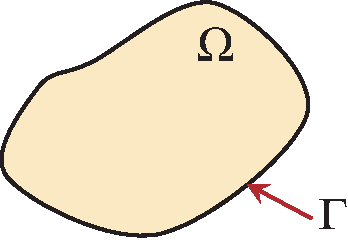
\includegraphics[width=0.6\linewidth]{pic/格林无点.pdf}
		\caption{空间区域}
		\label{格林3}
	\end{minipage}
	\begin{minipage}{0.33\linewidth}
		\centering
		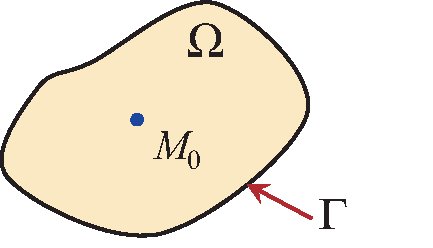
\includegraphics[width=0.6\linewidth]{pic/格林.pdf}
		\caption{空间区域内一点$M_0$}
		\label{格林4}
	\end{minipage}
	\begin{minipage}{0.33\linewidth}
	\centering
	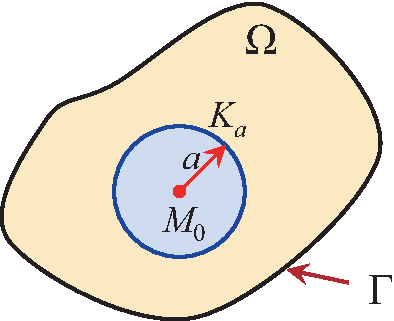
\includegraphics[width=0.5\linewidth]{pic/格林平均.pdf}
	\caption{调和函数的平均值}
	\label{格林5}
	\end{minipage}
\end{figure}

\noindent \textbf{2. 调和函数的积分表达式}

\theorem[三维Laplace方程的基本解]
球坐标形式的三维Laplace方程为
\begin{equation}
	\dfrac{1}{r^2}\dfrac{\partial }{\partial r}\left(r^2 \dfrac{\partial u}{\partial r}\right) + \dfrac{1}{r^2 \sin \theta} \dfrac{\partial }{\partial \theta}\left(\sin \theta \dfrac{\partial u}{\partial \theta}\right) + \dfrac{1}{r^2 \sin^2 \theta}\dfrac{\partial^2 u}{\partial \varphi^2} = 0
\end{equation}
此方程的三维球对称解$u = V(r)$满足$\dfrac{\d}{\d r}\left( r^2 \dfrac{\d V}{\d r} \right) = 0$,其通解为
\begin{equation}
	V(r) = \dfrac{c_1}{r} + c_2
\end{equation}
令$c_1 = 1, c_2 = 0$得到\dy[三维Laplace方程的基本解]{SWLAPLACEFCDJBJ}
\begin{equation}
	V_0(r) = \dfrac{1}{r}
\end{equation}

将基本解代入三维Laplace方程,则可以得到调和函数的积分表达式:

若函数$u$在$\Omega + \Gamma$上有一阶连续偏导数,且在$\Omega$内调和,则
\begin{equation}
	u(M_0) = - \dfrac{1}{4\pi} \iint\limits_{\Gamma}\Bigg[u(M)\dfrac{\partial }{\partial n} \left(\dfrac{1}{r_{MM_0}}\right) - \dfrac{1}{r_{MM_0}}\dfrac{\partial u(M)}{\partial n}\Bigg]\, \d S
\end{equation}
其中,$r_{MM_0} = \sqrt{(x - x_0)^2  + (y - y_0)^2 + (z-z_0)^2}.$

式子的含义:用$u$在$\Gamma $上的值和$u$在$\Gamma$上法向导数的值,来表达其在$\Omega$内任一点$M_0$的值,被称为\dy[调和函数的积分表达式]{THHSDJFBDS}。
\vspace*{1em}

\noindent \textbf{3. 平均值公式}

设函数$u(M)$在区域内调和,$M_0$是$\Omega$内任何一点,$K_a$表示以$M_0$为球心,以$a$为半径且完全落在区域$\Omega$内部的球面,则有\dy[平均值公式]{PJZGS}(球心值和球面平均值的关系)
\begin{equation}
	u(M_0) = \dfrac{1}{4 \pi a^2} \iint\limits_{K_a}u\, \d S
\end{equation}

证明:将积分表达式应用于球面$K_a$,注意到此时$r$的方向就是表面法向,再利用边界平衡性质即可。

\noindent \textbf{4. 极值原理}

设函数$u(x,y,z)$在区域内调和,在$\Omega + \Gamma$上连续且不为常数,则它的最大值和最小值只能在边界处达到。

推论:
\begin{itemize}
	\item Dirichlet问题
	$\begin{cases}
		\, \nabla^2 u = 0, \quad (x,y,z) \in \Omega\\
		\, u\big|_{\Gamma} = f
	\end{cases}$
	的解是唯一的。
	
	\item Neumann问题
	$
	\begin{cases}
		\, \nabla^2 u = 0, \quad (x,y,z) \in \Omega\\
		\dfrac{\partial u}{\partial n}\Bigg|_{\Gamma} = f
	\end{cases}
	$
	的解除了相差一个常数外也是唯一的。
\end{itemize}

\section{格林函数}
\subsection{格林函数的引入}
格林函数是为了解决Laplace方程的Dirichlet问题提出的
\begin{equation}
	\begin{cases}
		\, \nabla^2 u = 0, \quad (x,y,z) \in \Omega\\
		\, u\big|_{\Gamma} = f
	\end{cases}
\end{equation}
而调和函数的积分表达式
\begin{equation*}
	u(M_0) = - \dfrac{1}{4\pi} \iint\limits_{\Gamma}\Bigg[u(M)\dfrac{\partial }{\partial n} \left(\dfrac{1}{r_{MM_0}}\right) - \dfrac{1}{r_{MM_0}}\dfrac{\partial u(M)}{\partial n}\Bigg]\, \d S
\end{equation*}
并不能直接提供解,因为其边界上的值虽然已知,而法向导数的值却不知道,需要想办法消去。为此,提出格林函数。

设在$\Omega$内有$\nabla^2 u=0,\nabla^2 v = 0$;$u,v$在$\Omega + \Gamma$上有一阶连续偏导数,则由格林第二公式有
\begin{equation}
	\iiint\limits_{\Omega} \big(u \nabla^2 v - v \nabla^2 u\big)\, \d V = \iint\limits_{\Gamma} \Bigg(u\dfrac{\partial v}{\partial n} - v \dfrac{\partial u}{\partial n}\Bigg)\, \d S \quad \xrightarrow[\textstyle \nabla^2 v = 0]{\textstyle \quad \nabla^2 u = 0 \quad } \quad \iint \limits_{\Gamma}\Bigg(u\dfrac{\partial v}{\partial n} - v \dfrac{\partial u}{\partial n}\Bigg)\, \d S =  0
\end{equation}
再将这个式子与积分表达式相加得
\begin{equation}
	u(M_0) = \iint \limits_{\Gamma} \Biggl\{u\left[\dfrac{\partial v}{\partial n} - \dfrac{1}{4\pi}\dfrac{\partial }{\partial n}\left(\dfrac{1}{r_{MM_0}}\right)\right] + \left(\dfrac{1}{4\pi}\dfrac{1}{r_{MM_0}} - v\right)\dfrac{\partial u}{\partial n}\Biggr\}\, \d S
\end{equation}
为了消除$u$的法向导数,不妨选择调和函数$v$满足
\begin{equation}
	v\big|_\Gamma = \dfrac{1}{4\pi}\dfrac{1}{r_{MM_0}}\Bigg|_\Gamma
\end{equation}
所以
\begin{equation}
	u(M_0) = - \iint\limits_{\Gamma}u \dfrac{\partial }{\partial n}\left[\dfrac{1}{4\pi}\left(\dfrac{1}{r_{MM_0}}\right)-v\right]\, \d S
\end{equation}
引入\dy[格林函数]{GLHS}
\begin{equation}
	G(M,M_0) = \dfrac{1}{4\pi } \left(\dfrac{1}{r_{MM_0}}\right) - v
\end{equation}
则最终解可以表示为
\begin{equation}
	u(M_0) = - \iint\limits_{\Gamma} u \dfrac{\partial G}{\partial n}\, \d S
\end{equation}

整个格林函数的获得思路如图\ref{格林思路}.
\begin{figure}[!htb]
	\centering
	\begin{tikzpicture}
		\node (A) [draw, inner sep = 5pt]{高斯公式};
		\node (A1) [draw, inner sep = 5pt, right of = A, node distance = 7cm]{$\displaystyle \iiiint\limits_{\Omega} \nabla \cdot \vec{U}\, \d V = \iint\limits_{\Gamma}\vec{U}\cdot \, \d \vec{S}$};
		\node (B) [draw, inner sep = 5pt, below of = A, node distance = 2cm]{第二格林公式};
		\node (B1) [draw, inner sep = 5pt, right of = B, node distance = 8.45cm]{$\displaystyle \iiint\limits_{\Omega}\big(u \nabla^2 v - v\nabla^2 u\big)\, \d V = \iint\limits_{\Gamma}\Bigg(u\dfrac{\partial v}{\partial n}- v \dfrac{\partial u}{\partial n}\Bigg)\, \d S$};
		\node (C) [draw, inner sep = 5pt, below of = B, node distance = 2cm]{调和函数};
		\node (C1) [draw, inner sep = 5pt, right of = C, node distance = 9.25cm]{具有二阶连续偏导数并且满足Laplace方程的连续函数};
		\node (D) [draw, inner sep = 5pt, below of = C, node distance = 2cm]{调和函数的积分表达式};
		\node (D1) [draw, inner sep = 5pt, right of = D, node distance = 9.2cm]{$\displaystyle u(M_0) = - \dfrac{1}{4\pi}\iint\limits_{\Gamma} \Bigg[u(M)\dfrac{\partial }{\partial n}\left(\dfrac{1}{r_{MM_0}}\right) - \dfrac{1}{r_{MM_0}}\dfrac{\partial u(M)}{\partial n}\Bigg]\, \d S$};
		\node (E) [draw, inner sep = 5pt, below of = D, node distance = 3.65cm]{引入调和函数$v$};
		\node (E1) [inner sep = 5pt, right of = E, node distance = 4cm]{$
			\begin{cases}
				\, \nabla^2 v = 0, \quad (x,y,z) \in \Omega \\[0.5em]
				\, v\big|_\Gamma = \dfrac{1}{4\pi}\dfrac{1}{r_{MM_0}}\Bigg|_{\Gamma}
			\end{cases}
			$};
		\node (E2) [inner sep = 5pt, right of = E1, node distance = 5cm]{$G(M,M_0) = \dfrac{1}{4\pi} \left(\dfrac{1}{r_{MM_0}}\right) - v$};
		\node (E3) [draw, inner sep = 5pt, right of = E2, node distance = 4cm]{引入格林函数$G$};
		\node (F) [draw, inner sep = 5pt, below of = D1, node distance = 6.7cm, xshift = - 2.8cm]{$\displaystyle u(M_0) = -\iint\limits_{\Gamma} u \dfrac{\partial G}{\partial n}\, \d S$};
		\node (G) [draw, inner sep = 5pt, below of = F, node distance = 2.5cm]{$\displaystyle u(M_0) = - \iint \limits_{\Gamma} f\dfrac{\partial G}{\partial n}\, \d S$};
	
		
		\draw[arrows={-Stealth[scale=0.8]}] (A) -- (B);
		\draw[arrows={-Stealth[scale=0.8]}] (B) -- (C);
		\draw[arrows={-Stealth[scale=0.8]}] (C) -- (D);
		\draw[arrows={-Stealth[scale=0.8]}] (F) -- (G)node[midway, xshift = 2.6cm]{对于Dirichlet问题已知$u\big|_{\Gamma} = f$};
		\draw[arrows={-Stealth[scale=0.8]}] (D1) -- +(0cm, -1.5cm) --+(-2.8cm, -1.5cm) -- (F);
		\draw[dashed] (-1.9cm, -8.25cm) --+ (0cm,-2.8cm) -- +(16.8cm, -2.8cm) --+ (16.8cm, 0cm) --+ (0cm,0cm);
		
		\draw (A) -- (A1);
		\draw (B) -- (B1);
		\draw (C) -- (C1);
		\draw (D) -- (D1);
		\draw[arrows={-Stealth[scale=0.8]}] (E) -- (E1);
		\draw[arrows={-Stealth[scale=0.8]}] (E3) -- (E2);

	\end{tikzpicture}
	\vspace*{-0.5em}
	\caption{格林函数获得的思路图}
	\label{格林思路}
\end{figure}
\vspace*{-1em}

\warn[
\textbf{引入格林函数的意义}
\vspace*{-0.5em}
{
\begin{enumerate}[\hspace*{2em} 1. ]
	\item 将Laplace方程或泊松方程Dirichlet问题的求解,转化为求此区域内的格林函数。
	\item 求格林函数需要解定解问题
	$
	\begin{cases}
		\, \nabla^2 v = 0, \quad (x,y,z) \in \Omega \\[0.5em]
		\, v\big|_\Gamma = \dfrac{1}{4\pi}\dfrac{1}{r_{MM_0}}\Bigg|_{\Gamma}
	\end{cases}
	$进而$G(M,M_0) = \dfrac{1}{4\pi} \left(\dfrac{1}{r_{MM_0}}\right) - v$。
	\item 此问题只与区域有关,因此格林函数也只与区域有关。所以,只要求得了某个区域的格林函数,就能一劳永逸解决此区域上的一切边界条件的Dirichlet问题。
	\vspace*{-0.5em}
	
	\item 对于某些特殊的区域,如半空间、球等,格林函数可以用初等方法得到。
\end{enumerate}
}
]

\subsection{格林函数的性质}
格林函数
\begin{equation}
	G(M,M_0) = \dfrac{1}{4\pi} \left(\dfrac{1}{r_{MM_0}}\right) - v
\end{equation}
其中,函数$v$满足
\begin{equation}
	\begin{cases}
		\, \nabla^2 v = 0, \quad (x,y,z) \in \Omega \\[0.5em]
		\, v\big|_\Gamma = \dfrac{1}{4\pi}\dfrac{1}{r_{MM_0}}\Bigg|_{\Gamma}
	\end{cases}
\end{equation}
\vspace*{0.5em}

\begin{enumerate}[\textbf{性质} 1 \hspace*{1em}]
	\item 格林函数$G(M,M_0)$在去除$M=M_0$一点外处处满足Laplace方程,当$M \to M_0$时,$G(M,M_0)$趋于无穷大。
	
	\item 在边界$\Gamma$上格林函数恒等于0,即$G(M,M_0)\big|_\Gamma = 0.$
	
	\item 在区域$\Omega$内,下面不等式成立
	\begin{equation}
		0 < G(M,M_0) < \dfrac{1}{4\pi r_{MM_0}}
	\end{equation}
	
	\item 格林函数$G(M,M_0)$关于自变量$M$及参变量$M_0$之间具有对称性,即$G(M,M_0) = G(M_0, M).$
\end{enumerate}

\subsection{格林函数的静电学背景}
\begin{figure}[!htb]
	\centering
	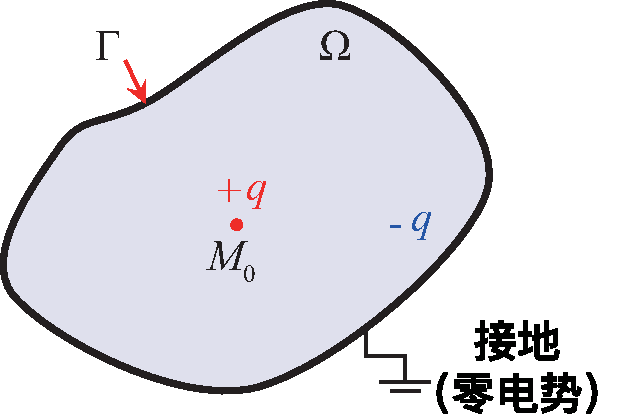
\includegraphics[width=0.3\linewidth]{pic/格林静电.pdf}
	\caption{格林函数的静电学背景}
	\label{格林静电}
\end{figure}

如图\ref{格林静电},考虑空腔$\Omega$,容器壁$\Gamma$为导体,其内部一点$M_0$存在单位正电荷$+q$。

根据静电学知识,此时内壁因静电感应出现等值异号电荷$-q$,外壁由电荷守恒产生感应电荷$+q$,整个壁面为等势面。

再进一步,令容器壁接地,此时外侧正电荷消失,壁面为零电势。且容器内任何一点电势,就是点电荷的电势和内表面感生电荷电势的叠加。所以,壁面为零电势是感生电荷电势抵消点电荷电势的结果。

\textbf{格林函数各项的静电学意义}
\begin{enumerate}[\hspace*{2em} 1. ]
	\item $\dfrac{1}{4 \pi r_{MM_0}}$\quad $M_0$点处的单位正电荷在无界空间中产生的电势
	\item $-v$ \quad 感生负电荷引起的电势
	\item $G(M,M_0)$ \quad 接地容器内的实际电势:单位正电荷电势$+$内壁感生负电荷电势
\end{enumerate}

所以,格林函数$G(M,M_0)$是在接地导电容器内$M_0$点放置单位正点电荷后的电势分布。因此,格林函数又被称为\dy[点源函数]{DYHS}。

\section{两种特殊区域的格林函数及 Dirichlet 问题的解}
\subsection{电像法}
边界零电势,除了可以由 真实情况下的内部感生电荷实现外,还可以通过引入外部虚拟点电荷的方式来满足,这是电像法的物理基础。利用真实内部感生电荷和外部虚拟点电荷的等效性,转化
为虚拟点电荷问题,实现求解的方法称为\dy[电像法]{DXF}。
\vspace*{0.5em}

\noindent \textbf{电像法的基本操作步骤}
\begin{enumerate}[\hspace*{2em} 1. ]
	\item 在区域外找出区域内点$M_0$关于边界的像点。\vspace*{-0.5em}
	\item 放置适量负点电荷,和原内壁感生电荷起到的效果完全相同,即边界零电势。\vspace*{-0.5em}
	\item 叠加后在区域中形成的电势场就是所要求的格林函数。
\end{enumerate}

\subsection{半空间的格林函数法}
用格林函数法解定解问题
\begin{equation}
	\begin{cases}
		\, \dfrac{\partial^2 u}{\partial x^2} + \dfrac{\partial^2 u}{\partial y^2} + \dfrac{\partial^2 u}{\partial z^2} = 0, & z > 0\\[0.5em]
		\, u\big|_{z=0} = f(x,y),& -\infty < x,y<+\infty
	\end{cases}
\end{equation}

\solve 运用电像法求解。
\begin{enumerate}[\textbf{步骤} 1 ]
	\item \textbf{求解格林函数}
	
	物理含义\quad 上半空间$z>0$一点$M_0$放置单位正电荷,再将导电平面$z=0$接地后,上半平面的电势分布。
	
	电像法\quad 在下半平面镜像位置放置单位负电荷后撤去平板。
	\vspace*{0.5em}
	\begin{figure}[!htb]
		\centering
		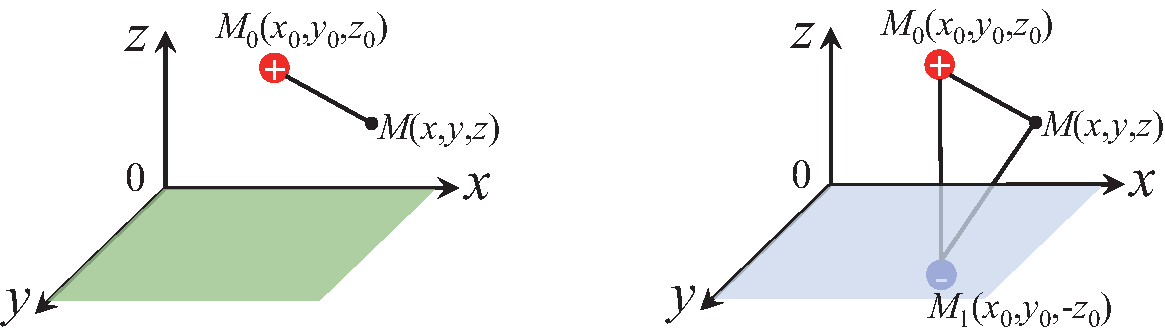
\includegraphics[width=0.8\linewidth]{pic/格林半平面.pdf}
		\caption{半空间的格林函数及其电像法}
		\label{格林半平面}
	\end{figure}
	\vspace*{-0.5em}
	
	如图\ref{格林半平面},在上半平面一点$M_0(x_0,y_0,z_0)$放置单位正电荷,在其关于平面$z=0$的镜像点$M_1(x_0,y_0,-z_0)$放置单位负电荷,同时撤去$z = 0$处的导体平面。
	
	由于$\dfrac{1}{4\pi r_{MM_0}}$表示点$M_0$处的单位正电荷在无界空间中产生的电势,
	
	那么$-\dfrac{1}{4\pi r_{MM_1}}$就表示点$M_1$处的单位负电荷在无界空间中产生的电势,则半空间$z>0$的格林函数就是:
	\begin{equation}
		G(M,M_0) = \dfrac{1}{4\pi r_{MM_0}} - \dfrac{1}{4\pi r_{MM_1}}
	\end{equation}

	\item \textbf{得到定解问题的解}
	
	已知格林函数,定解问题的解可表示为
	\begin{equation}
		u(M_0) = - \iint \limits_{\Gamma} f(M)\dfrac{\partial G}{\partial n}\, \d S
	\end{equation}
	其中,$\Gamma$为平面$z = 0$,外法线方向为$-z$方向,则
	\begin{align*}
		\dfrac{\partial G}{\partial n}\Bigg|_{z = 0} = - \dfrac{\partial G}{\partial z}\Bigg|_{z = 0} &=
		\left \lbrace\dfrac{1}{4\pi}\dfrac{z-z_0}{\big[(x-x_0)^2 + (y-y_0)^2 + (z-z_0)^2\big]^{\textstyle \frac{3}{2}}} -\dfrac{1}{4\pi}\dfrac{z+z_0}{\big[(x-x_0)^2 + (y-y_0)^2 + (z+z_0)^2\big]^{\textstyle \frac{3}{2}}} \right \rbrace\\[0.5em]
		& = -\dfrac{1}{2\pi} \dfrac{z_0}{\big[(x-x_0)^2 + (y-y_0)^2 + z_0^2\big]^{\textstyle \frac{3}{2}}}
	\end{align*}
	所以最终解为
	\begin{align}
		u(M_0) & = - \iint\limits_{\Gamma}f(M) \dfrac{\partial G}{\partial n}\, \d S \notag \\[0.5em]
		& = \dfrac{1}{2\pi} \int_{-\infty}^{+\infty}\int_{-\infty}^{+\infty} \dfrac{z_0f(x,y)}{\big[(x-x_0)^2 + (y-y_0)^2 + z_0^2\big]^{\textstyle \frac{3}{2}}}\, \d x \d y
	\end{align}
\end{enumerate}

\subsection{球域的格林函数法}
用格林函数法解定解问题
\begin{equation}
	\begin{cases}
		\, \dfrac{\partial^2 u}{\partial x^2} + \dfrac{\partial^2 u}{\partial y^2} + \dfrac{\partial^2 u}{\partial z^2} = 0, & x^2+y^2+z^2 < R^2\\[0.5em]
		\, u\big|_{x^2 + y^2 + z^2=R^2} = f(x,y,z),& x^2 + y^2 + z^2=R^2
	\end{cases}
\end{equation}

\solve 运用电像法求解。
\begin{enumerate}[\textbf{步骤} 1 ]
	\item \textbf{求解格林函数}
	
	物理含义\quad 在球内一点$M_0$放置单位正电荷,再将导电平面$z=0$接地后,球内的电势分布。
	
	电像法\quad 在球面外部位置放置适量的负电荷后撤去球面。
	\vspace*{0.5em}
	\begin{figure}[!htb]
		\centering
		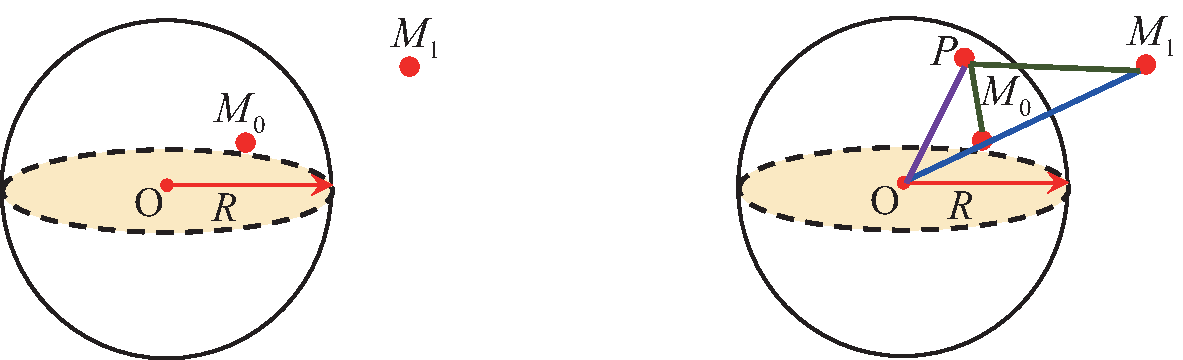
\includegraphics[width=0.8\linewidth]{pic/格林球域.pdf}
		\caption{球域的格林函数及其电像法}
		\label{格林球域}
	\end{figure}
	\vspace*{-0.5em}
	
	如图\ref{格林球域},由于球面的复杂性,负电荷的放置位置以及电荷量$q$不能直接观测得到。由物理学的知识可知,$M_1$应满足在线段$OM_0$的延长线上,且满足$r_{OM_0}\cdot r_{OM_1} = R^2$.
	
	而负电荷量的大小$q$需使得球面处叠加电势为0,即$\dfrac{1}{4 \pi r_{PM_0}} = \dfrac{q}{4\pi r_{PM_1}}$,$P$为球面上的点,即$q = \dfrac{r_{PM_1}}{r_{PM_0}}$.
	
	\begin{equation}
		\begin{cases}
			\, \dfrac{r_{OM_0}}{R} = \dfrac{R}{r_{OM_1}}\\
			\, \angle POM_1 = \angle POM_0
		\end{cases}
		\quad \Rightarrow \quad 
		\triangle OPM_1 \sim \triangle OM_0P \quad \Rightarrow \quad 
		q = \dfrac{r_{PM_1}}{r_{PM_0}} = \dfrac{R}{r_{OM_0}}
	\end{equation}
	由电势叠加,得到格林函数
	\begin{equation}
		G(M,M_0) = \dfrac{1}{4\pi} \Bigg(\dfrac{1}{r_{MM_0}}- \dfrac{R}{r_{OM_0}}\dfrac{1}{r_{MM_1}} \Bigg)
	\end{equation}
	
	\item \textbf{得到定解问题的解}
	
	已知格林函数,定解问题的解可表示为
	\begin{equation}
		u(M_0) = - \iint \limits_{\Gamma} f(M)\dfrac{\partial G}{\partial n}\, \d S
	\end{equation}
	其中,$\Gamma$为半径为$R$的球面,外法线方向为球心指向外的射线方向,记为变量$r_{OM}$,则
	\begin{equation}
		\begin{cases}
			\, r_{MM_0} = \sqrt{r_{OM}^2+r_{OM_0}^2 - 2 r_{OM}r_{OM_0}\cos \gamma} \\[0.5em]
			\, r_{MM_1} = \sqrt{r_{OM}^2+r_{OM_1}^2 - 2 r_{OM}r_{OM_1}\cos \gamma} 
		\end{cases}
		\quad \quad \gamma = \big<\overrightarrow{OM_0}, \overrightarrow{OM}\big>
	\end{equation}
	进一步得到格林函数
	\begin{equation}
		G(M,M_0) = \dfrac{1}{4\pi} \left(\dfrac{1}{\sqrt{r_{OM}^2+r_{OM_0}^2 - 2 r_{OM}r_{OM_0}\cos \gamma}} - \dfrac{R}{\sqrt{r_{OM}^2+r_{OM_1}^2 - 2 r_{OM}r_{OM_1}\cos \gamma}} \right)
	\end{equation}
	所以,
	\begin{align*}
		\dfrac{\partial G}{\partial n}\Bigg|_{\Gamma} &= \dfrac{\partial G}{\partial r_{OM}}\Bigg|_{r_{OM} = R}\\[0.5em]
		& = \dfrac{1}{4\pi} \dfrac{\partial }{\partial r_{OM}} \left(\dfrac{1}{\sqrt{r_{OM}^2+r_{OM_0}^2 - 2 r_{OM}r_{OM_0}\cos \gamma}} - \dfrac{R}{\sqrt{r_{OM}^2+r_{OM_1}^2 - 2 r_{OM}r_{OM_1}\cos \gamma}} \right)_{r_{OM} = R}\\[0.5em]
		& = -\dfrac{1}{4\pi R} \dfrac{R^2-r_{OM_0}^2}{\big(R^2 + r_{OM_0}^2 - 2Rr_{OM_0} \cos \gamma\big)^{\textstyle \frac{3}{2}}}
	\end{align*}
	得到最终解为
	\begin{align}
		u(M_0) & = - \iint\limits_{\Gamma}f(M) \dfrac{\partial G}{\partial n}\, \d S \notag \\[0.5em]
		& = \dfrac{1}{4\pi R}\iint\limits_{\Gamma} \dfrac{\big(R^2-r_{OM_0}^2\big)f(x,y,z)}{\big(R^2 + r_{OM_0}^2 - 2Rr_{OM_0} \cos \gamma\big)^{\textstyle \frac{3}{2}}}\, \d S\\[0.5em]
		& = \dfrac{R}{4\pi}\int_0^{2\pi}\int_0^{\pi} f(R, \theta, \varphi) \dfrac{R^2 - r_0^2}{\big(R^2+r_0^2 -2Rr_0\cos \gamma \big)^{\textstyle \frac{3}{2}}} \sin \theta \, \d \theta \d \varphi
	\end{align}
	其中,$(r_0,\theta_0,\varphi_0)$是点$M_0$的球坐标,$(R,\theta, \varphi)$是球面$\gamma $上任意一点$P$的坐标,$\gamma$是$OP,OM_0$的夹角,也可以表示为
	\begin{equation}
		\cos \gamma = \cos \theta \cos \theta_0 + \sin \theta \sin \theta_0 \cos(\varphi - \varphi_0)
	\end{equation}
\end{enumerate}





















